\chapter{Конструкторский раздел}
\label{cha:design}

В данном разделе будут описаны особенности аппаратной платформы STM32, а также алгоритмы и структуры данных, выбранные для решения 
поставленной задачи, будет разработана структура программного комплекса.

\section{Особенности архитектуры ARM}

\textbf{Архитектура ARM} — система команд и семейство описаний и готовых топологий 32-битных и 64-битных микропроцессорных/микроконтроллерных ядер.

Архитектура развивалась с течением времени и, начиная с ARMv7, были определены три профиля: для устройств, требующих высокой производительности (смартфоны, планшеты), для приложений, работающих в реальном времени, и для микроконтроллеров и бюджетных встраиваемых устройств \cite{ARM_dev_doc}.

Основные отличия архитектуры ARM от x86, которая используется в современных ПК: \cite{ARM_vs_x86} % Помогите, я не знаю, в каком месте эту ссылку надо воткнуть...
\begin{itemize}
	\item использование упрощенного набора инструкций - \textbf{RISC} (Reduced Instruction Set Computing);
	\item предикация - возможность условного исполнения практически любой команды;
	\item упрощённая работа с памятью за счёт использования единого адресного пространства для всех устройств вычислительной машины;
	\item более объёмная регистровая архитектура \cite{ARM_registers} \cite{x86_registers};
	\item меньшее энергопотребление;
	\item системы, базирующиеся на процессорах ARM, проще масштабировать и отлаживать.
\end{itemize}

Архитектура ARM поддерживается множеством операционных систем, к числу которых относятся Linux (в том числе Android, основанная на ядре ОС Linux), iOS, BSD, macOS Big Sur. Также на платформе запускаются отдельные варианты семейства ОС Windows: Windows CE, Windows Phone, Windows RT, Windows 10.

Процессоры ARM широко используются в потребительской электронике, к которой относятся смартфоны, плееры, портативные игровые консоли, калькуляторы, умные часы и компьютерные периферийные устройства. Эти процессоры имеют низкое энергопотребление, поэтому находят широкое применение во встраиваемых системах и преобладают на рынке мобильных устройств, для которых данный фактор критически важен \cite{ARM_consumers}.

\section{Описание семейства микроконтроллеров STM32}
Многие лицензиаты готовых топологий ядер ARM проектируют собственные топологии ядер на базе системы команд ARM. Одной из таких компаний является STMicroelectronics, производящая различные полупроводниковые электронные и микроэлектронные компоненты, к которым относятся микроконтроллеры семейства STM32.

\textbf{STM32} — семейство микроконтроллеров, основанных на 32-битных ядрах ARM Cortex-M. Каждый микроконтроллер состоит из ядра процессора, статической RAM-памяти, флеш-памяти, отладочного и различных периферийных интерфейсов.

Дизайн ядра ARM имеет множество настраиваемых опций, и для каждого микроконтроллера выбирается индивидуальная конфигурация с добавлением своих собственных периферийных устройств к ядру микроконтроллера перед преобразованием дизайна в полупроводниковую пластину.

Основные преимущества микроконтроллеров STM32:
\begin{itemize}
	\item низкая стоимость;
	\item гибкая и масштабируемая экосистема;
	\item большой выбор сред разработки;
	\item высокая производительность;
	\item наличие инструментов для отладки микроконтроллера.
\end{itemize}

Самым важным преимуществом STM32 является взаимозаменяемость чипов, которая достигается за счёт универсальности ядра STM32, позволяющего менять производителя c минимальными затратами на программный код. Также внутри семейства STM32 поддерживается pin-to-pin совместимость, которая позволяет менять объем памяти (флэш-память и ОЗУ) и периферию (Ethernet, USB, CAN и так далее), не меняя печатную плату. Таким образом, если для решения какой-либо задачи не хватает ресурсов одного микроконтроллера, его можно заменить на более мощный, не меняя самой схемы и платы \cite{STM32_advantages}.

\section{Структуры данных}
Чтобы формализовать алгоритм синтеза изображения в программе, необходимо определить структуры данных, которые будут в ней использоваться. 
% Итак, будем считать, что
В данной работе приняты следующие соглашения:
\begin{enumerate}
	\item[1)] трёхмерные модели являются полигональными, тогда сцену можно представить в виде массива многоугольников (полигонов);
	\item[2)] многоугольник включает в себя следующие данные:
	\begin{itemize}
		\item количество вершин;
		\item массив x и y координат вершин;
		\item коэффициенты уравнения поверхности, несущей данный многоугольник, заданного в виде $a*x + b*y + c*z = 1000$;
		\item цвет;
	\end{itemize}
	\item[3)] окна, использующиеся в алгоритме Варнока, имеют прямоугольную форму и хранят следующую информацию:
	\begin{itemize}
		\item количество многоугольников, рассматриваемых при изображении данного окна;
		\item массив многоугольников;
		\item координаты x и y левой нижней и правой верхней вершин окна.
	\end{itemize}
\end{enumerate}

\section{Разработка алгоритмов}
\subsection{Алгоритм работы программы}
Диаграмма, оформленная в соответствии с нотацией IDEF0 и отражающая общую декомпозицию алгоритма работы программы, представлена в 
приложении \ref{cha:appendix1}.


\subsection{Алгоритм Варнока}

Для удаления невидимых линий и поверхностей был выбран алгоритм Варнока, основанный на рекурсивном разбиении окон. Под окном в данном 
алгоритме понимается область изображения на дисплее, которая может содержать визуализируемые объекты сцены. Разбиение окон в алгоритме 
Варнока может быть реализовано как рекурсивно, так и итерационно. В данной работе будет рассматриваться итерационная реализация с 
использованием стека окон, так как она задействует меньший объём памяти, чем рекурсивная. Максимальная длина стека окон составляет
\begin{equation}
]\log_{2} (max(w; h))[ + 2 * (]\log_{2} (min(w; h))[ + 1) + 2,
\label{F:F1}
\end{equation}
где w – горизонтальное разрешение дисплея, h – вертикальное разрешение дисплея.

Схема алгоритма Варнока представлена в приложении \ref{cha:appendix2} на рисунке \ref{fig:warnock_algorithm} На рисунке 
\ref{fig:warnock_identification} представлен алгоритм идентификации взаимного расположения окна и рассматриваемого многоугольника. Алгоритм 
следует оформить в виде подпрограммы.

\section{Структура программного комплекса}
На рисунке \ref{fig:deploy_diagram} представлена структура программного комплекса, оформленная в виде диаграммы развёртывания. Она отражает компоненты, необходимые для работы системы, а также способы их взаимодействия.

\begin{figure}[h]
	\centering
	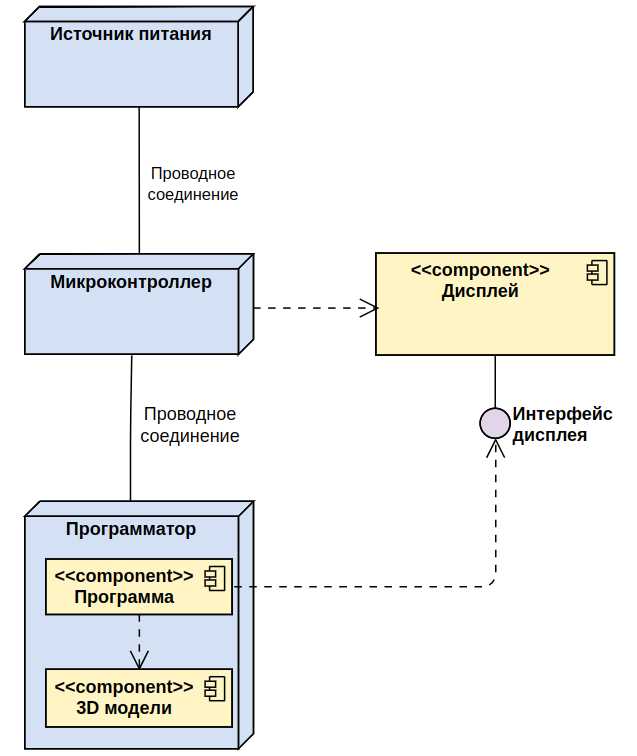
\includegraphics[scale=0.777 ]{img/deploy_diagram/dd1.png}
	\caption{Диаграмма развёртывания программного комплекса}
	\label{fig:deploy_diagram}
\end{figure} 

\section{Вывод из конструкторского раздела}
В данном разделе были описаны особенности работы с аппаратной платформой STM32, структура программного комплекса, а также алгоритмы и 
структуры данных, выбранные для решения поставленной задачи и отвечающие требованиям компактности, простоты и быстродействия.
%\begin{lstlisting}[style=pseudocode,caption={Алгоритм Флойда-Стейнберга и белый шум}]
%for x in range(width):
%    for y in range(height):
%        P(x,y) = trunc(I(x,y)+0.5)
%        e = I(x,y) - P(x,y)
%        I(x,y+1) += random.randint(1,alpha*16)/16*e
%        I(x+1, y-1) += random.randint(1,beta*16)/16*e
%        I(x+1, y) += random.randint(1,gamma*16)/16*e
%        I(x+1, y+1) +=  random.randint(1,sigma*16)/16*e
%\end{lstlisting}


%%% Local Variables:

%%% mode: latex
%%% TeX-master: "rpz"
%%% End:
%--количество цветов
%||количество пикселей